% !TEX program = xelatex
% Figure 1 (CONSORT 형식) — 환자 선정 흐름도. 흰 상자 + 검은 실선 + 왼쪽 제외 상자, Times New Roman.
% 서체: Times New Roman 은 ~/.local/share/fonts 에 사용자 설치(저장소에 넣지 말 것 — MS 라이선스).
%       없는 장비에서는 같은 Times 계열 Nimbus Roman 으로 자동 대체된다.
% 수치 출처(2026-10-06 재계산):
%   321 / 64 / 9 / 8 / 2 -> 238   src/sclc/cohort.py::build_manifest()  (fig1_patient_flowchart.tex 와 같음)
%   LS 72, ES 166                  merged_tabular_with_reports.csv 'stage' (1 = LS, 2 = ES)
%   fold 크기·사건 수               data/splits/trimodal_common_5fold_seed42_v1.csv + os_event/pfs_event
%     train 171 (OS 142-143, PFS 152-153) / val 19-20 (OS 16-17, PFS 17-18) / test 47-48 (OS 39-40, PFS 42-43)
\documentclass[tikz,border=8pt,10pt]{standalone}
\usepackage{fontspec}
\IfFontExistsTF{Times New Roman}{\setmainfont{Times New Roman}}{\setmainfont{Nimbus Roman}}
\usetikzlibrary{arrows.meta,positioning}
\begin{document}
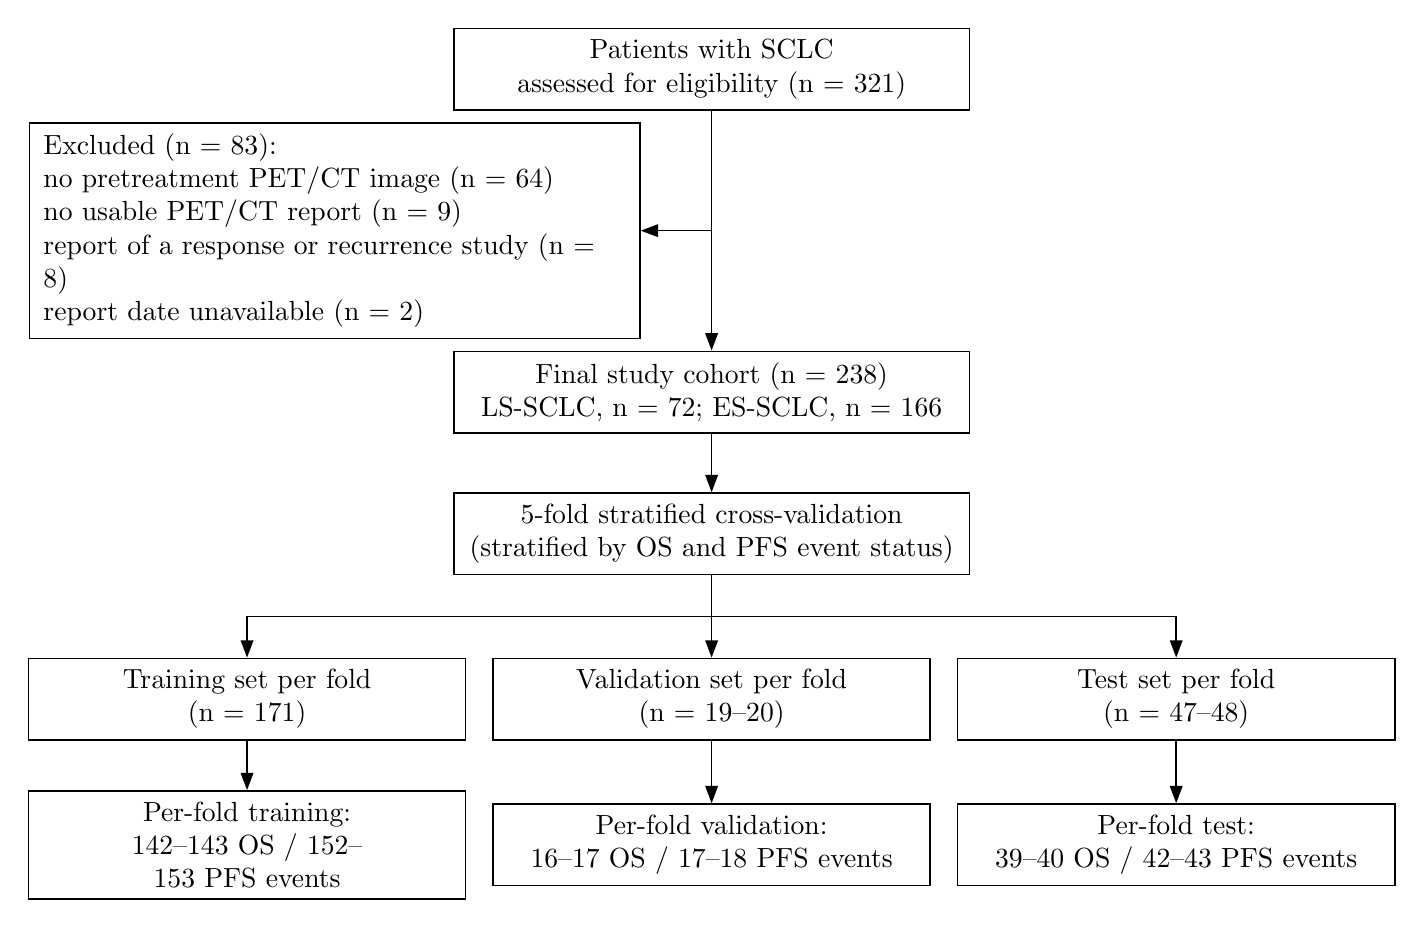
\begin{tikzpicture}[x=1cm,y=1cm,
  box/.style={draw=black, line width=0.6pt, fill=white, align=center,
              inner xsep=5pt, inner ysep=4pt, text width=#1},
  box/.default=62mm,
  excl/.style={box=74mm, align=left},
  sub/.style={box=52mm},
  arr/.style={draw=black, line width=0.6pt, -{Triangle[length=2.2mm,width=1.6mm]}},
  line/.style={draw=black, line width=0.6pt},
]

% ---------------- 선정 ----------------
\node[box] (all) at (0,0)
  {Patients with SCLC\\ assessed for eligibility (n = 321)};

\node[excl, anchor=east] (ex) at (-0.9,-2.05)
  {Excluded (n = 83):\\
   no pretreatment PET/CT image (n = 64)\\
   no usable PET/CT report (n = 9)\\
   report of a response or recurrence study (n = 8)\\
   report date unavailable (n = 2)};

\node[box] (final) at (0,-4.1)
  {Final study cohort (n = 238)\\ LS-SCLC, n = 72; ES-SCLC, n = 166};

% ---------------- 교차검증 ----------------
\node[box] (cv) at (0,-5.9)
  {5-fold stratified cross-validation\\ (stratified by OS and PFS event status)};

\node[sub] (tr) at (-5.9,-8.0) {Training set per fold\\ (n = 171)};
\node[sub] (va) at (0,-8.0)    {Validation set per fold\\ (n = 19--20)};
\node[sub] (te) at (5.9,-8.0)  {Test set per fold\\ (n = 47--48)};

\node[sub] (trd) at (-5.9,-9.85) {Per-fold training:\\ 142--143 OS / 152--153 PFS events};
\node[sub] (vad) at (0,-9.85)    {Per-fold validation:\\ 16--17 OS / 17--18 PFS events};
\node[sub] (ted) at (5.9,-9.85)  {Per-fold test:\\ 39--40 OS / 42--43 PFS events};

% ---------------- 화살표 ----------------
\draw[arr] (all) -- (final);
\draw[arr] (0,-2.05) -- (ex.east);
\draw[arr] (final) -- (cv);

\coordinate (fork) at (0,-6.95);
\draw[line] (cv.south) -- (fork);
\draw[line] (-5.9,-6.95) -- (5.9,-6.95);
\draw[arr] (-5.9,-6.95) -- (tr.north);
\draw[arr] (fork) -- (va.north);
\draw[arr] (5.9,-6.95) -- (te.north);

\draw[arr] (tr) -- (trd);
\draw[arr] (va) -- (vad);
\draw[arr] (te) -- (ted);

\end{tikzpicture}
\end{document}
